% Paquets généraux
\documentclass[a4paper,12pt,titlepage,twoside]{article}
\usepackage[T1]{fontenc}
\usepackage[utf8]{inputenc}
\usepackage[french]{babel}
\usepackage{subcaption}
\addto\captionsfrench{%
  \renewcommand{\tablename}{Tableau}%
}
\usepackage[gen]{eurosym}
%\usepackage[dvips]{graphicx}
\usepackage{minted}
\usepackage{fancyhdr}
\usepackage{pdfpages} 
\usepackage{multido}
\usepackage{hyperref}
\usepackage{textcomp}
\usepackage{schemabloc}
%\usepackage[bitstream-charter]{mathdesign}
\usepackage{array}
\newcolumntype{P}[1]{>{\centering\arraybackslash}p{#1}}
\usepackage[shortlabels]{enumitem}
\usepackage[framemethod=TikZ]{mdframed}

\newcommand{\id}{30}
\newcommand{\nom}{Calculs d'hyperstatisme}
\newcommand{\sequence}{04}
\newcommand{\nomsequence}{Liaisons entre les solides}
\newcommand{\num}{03}
\newcommand{\type}{TD}
\newcommand{\descrip}{En appliquant les règles de la théorie des mécanisme, déterminer le degré d'hyperstatisme de plusieurs systèmes et proposer des solutions afin de diminuer ce degré}
\newcommand{\competences}{B2-12: Proposer une modélisation des liaisons avec leurs caractéristiques géométriques. \\ &  B2-13: Proposer un modèle cinématique paramétré à partir d'un système réel, d'une maquette numérique ou d'u \\ &  B2-17: Simplifier un modèle de mécanisme. \\ &  B2-18: Modifier un modèle pour le rendre isostatique.}
\newcommand{\nbcomp}{4}
\newcommand{\systemes}{E.P.A.S, Machine d'essai de traction}
\newcommand{\systemesnum}{14, 13}
\newcommand{\systemessansaccent}{E.P.A.S, Machine d'essai de traction}
\newcommand{\ilot}{3}
\newcommand{\ilotstr}{03}
\newcommand{\dossierilot}{\detokenize{Ilot_03 E.P.A.S, Machine d'essai de traction}}
\newcommand{\imageun}{EPAS}
\newcommand{\imagedeux}{Machine_dessai_de_traction}

%\usepackage{style}
\usepackage{bodegraph}
\usepackage{rpcinematik}
\usepackage[locale = FR]{siunitx}
\usepackage{caption}
\newcommand{\institute}{Lycée Dorian}
\usepackage{calc}

\usepackage{listings}
\usepackage{fancyvrb}
\usepackage{color}
\usepackage{xcolor}
\usepackage{colortbl}
\usepackage{helvet}
\usepackage[frenchmath]{newtxsf} % for sans serif symbols
\renewcommand{\familydefault}{\sfdefault}
%\usepackage{amsfonts}
%\usepackage{amsmath}
%\usepackage{lmodern}
\usepackage{mathastext}
%\usepackage{xspace}
\usepackage{varioref}
\usepackage{tabularx}
%\usepackage{floatflt}
\usepackage{graphics}
\usepackage{wrapfig}
\usepackage{textcomp}
\usepackage{tikz,tkz-tab}
\usepackage[european resistor, european voltage, european current]{circuitikz}
\usepackage{wrapfig}
\usepackage{gensymb}
\usepackage[percent]{overpic}
\usetikzlibrary{babel}
\usepackage{ifthen}
\usepackage{cancel}
\usepackage{etoolbox}
\usepackage{multirow}
%\usepackage{boxedminipage}
\definecolor{gris25}{gray}{0.75}
\definecolor{bleu}{RGB}{18,33,98}
\definecolor{bleuf}{RGB}{42,94,171}
\definecolor{bleuc}{RGB}{231,239,247}
\definecolor{bleum}{RGB}{160,195,226}
\definecolor{rougef}{RGB}{185,18,27}
\definecolor{rougec}{RGB}{255,188,204}%255,230,231
\definecolor{vertf}{RGB}{103,126,82}
\definecolor{vertc}{RGB}{220,255,191}
\definecolor{forestgreen}{rgb}{0.13,0.54,0.13}
\definecolor{blcr}{rgb}{0.59,0.69,0.84}
\definecolor{blfr}{rgb}{0.32,0.51,0.75}
\definecolor{orfr}{rgb}{0.90,0.42,0.15}
\definecolor{orcr}{rgb}{0.90,0.65,0.50}
\definecolor{orangef}{rgb}{0.659,0.269,0.072}
\definecolor{orange}{rgb}{0.58,0.35,0.063}
\definecolor{orangec}{rgb}{0.43,0.32,0.25}
\definecolor{rcorrect}{rgb}{0.6,0,0}
\definecolor{sequence}{rgb}{0.75,0.75,0.75}
\definecolor{competences}{rgb}{0.61,0.73,0.35}
\definecolor{rose}{HTML}{ff00ff}
\definecolor{grisf}{HTML}{222222}
\definecolor{grisc}{HTML}{636363}
\definecolor{normal}{HTML}{4087c4}
\definecolor{info}{HTML}{5bc0de}
\definecolor{success}{RGB}{92,184,92}
\definecolor{warning}{RGB}{240,173,78}
\definecolor{danger}{RGB}{217,83,79}
\hypersetup{                    % parametrage des hyperliens
    colorlinks=true,                % colorise les liens
    breaklinks=true,                % permet les retours à la ligne pour les liens trop longs
    urlcolor= blfr,                 % couleur des hyperliens
    linkcolor= orange,                % couleur des liens internes aux documents (index, figures, tableaux, equations,...)
    citecolor= forestgreen                % couleur des liens vers les references bibliographiques
    }

\newcolumntype{M}[1]{>{\centering\arraybackslash}m{#1}}
\definecolor{codegreen}{rgb}{0,0.6,0}
\definecolor{codegray}{rgb}{0.5,0.5,0.5}
\definecolor{codepurple}{rgb}{0.58,0,0.82}
\definecolor{backcolour}{rgb}{0.95,0.95,0.92}

\lstdefinestyle{mystyle}{
    backgroundcolor=\color{backcolour},   
    commentstyle=\color{codegreen},
    keywordstyle=\color{magenta},
    numberstyle=\tiny\color{codegray},
    stringstyle=\color{codepurple},
    basicstyle=\ttfamily\footnotesize,
    breakatwhitespace=false,         
    breaklines=true,                 
    captionpos=b,                    
    keepspaces=true,                 
    numbers=left,                    
    numbersep=5pt,                  
    showspaces=false,                
    showstringspaces=false,
    showtabs=false,                  
    tabsize=2
}

\lstset{style=mystyle}

% Mise en page
\pagestyle{fancy}

\setlength{\hoffset}{-18pt}
\setlength{\oddsidemargin}{0pt} 	% Marge gauche sur pages impaire2s
\setlength{\evensidemargin}{0pt} 	% Marge gauche sur pages paires
\setlength{\marginparwidth}{00pt} 	% Largeur de note dans la marge
\setlength{\headwidth}{481pt} 	 	% Largeur de la zone de tête (17cm)
\setlength{\textwidth}{481pt} 	 	% Largeu\textbf{r de la zone de texte (17cm)
\setlength{\voffset}{-18pt} 		% Bon pour DOS
\setlength{\marginparsep}{7pt}	 	% Séparation de la marge
\setlength{\topmargin}{-30pt} 		% Pas de marge en haut
\setlength{\headheight}{55pt} 		% Haut de page
\setlength{\headsep}{20pt} 		% Entre le haut de page et le texte
\setlength{\footskip}{30pt} 		% Bas de\textbf{ page + séparation
\setlength{\textheight}{700pt} 		% Hauteur de l'icone zone de texte (25cm)
\setlength\fboxrule{1 pt}
\renewcommand{\baselinestretch}{1}
\setcounter{tocdepth}{1}
\newcommand{\cadre}[2]
{\fbox{
  \begin{minipage}{#1\linewidth}
   \begin{center}
    #2\\
   \end{center}
  \end{minipage}
 }
}

\newcommand{\repon}[1]
{
~\ \\
\begin{tabular}{|m{\linewidth}|}
 \hline
\multido{}{#1}{\\ \hline}
\end{tabular}
}


\newcommand{\objectif}[1]{
\mdfsetup{%
frametitle={%
\tikz[baseline=(current bounding box.east),outer sep=0pt]
\node[anchor=east,rectangle,fill=bleum]
{\strut Objectif~};}}
\mdfsetup{innertopmargin=10pt,linecolor=bleum,%
linewidth=2pt,topline=true,%
frametitleaboveskip=\dimexpr-\ht\strutbox\relax
}
\begin{mdframed}[]\relax%
#1
\end{mdframed}}


\newcounter{num_quest} \setcounter{num_quest}{0}
\newcounter{num_rep} \setcounter{num_rep}{0}
\newcounter{num_cor} \setcounter{num_cor}{0}

\newcommand{\feuilleDR}[1]{
	\begin{tikzpicture}
		\draw[gray!30](0,0)grid[step=0.5cm](\linewidth,#1);
	\end{tikzpicture}
}

%\newcommand{\question}[1]{\refstepcounter{num_quest}\par
%~\ \\ \parbox[t][][t]{0.15\linewidth}{\textbf{Question \arabic{num_quest}}}\parbox[t][][t]{0.85\linewidth}{#1\label{q\the\value{num_quest}}}\par
%}

\newcommand{\question}[1]{\refstepcounter{num_quest}\par
~\ \\ \textbf{Question \arabic{num_quest} : }#1\label{q\the\value{num_quest}}\par
}

\newcommand{\posetafigure}[3]{
\begin{figure}[ht!]
 \begin{center}
  \includegraphics[width=#2\linewidth]{img/#1}
 \end{center}
 \caption{\label{#1} #3}
\end{figure}}

\newcommand{\goforum}{
\begin{figure}

\end{figure}
\begin{center}
 \includegraphics[width=0.7\linewidth]{../../../img/go_forum}
\end{center}
\label{go_forum}
\caption{J'pète les plombs}
\end{figure}}

\newcommand{\reponse}[4][1]
{\noindent
\parbox{\textwidth}{
\rule{\linewidth}{.5pt}\\
\textbf{Question\ifthenelse{#1>1}{s}{} \multido{}{#1}{%
\refstepcounter{num_rep}\ref{q\the\value{num_rep}} }:} ~\ \\
\ifdef{\public}{#3 \ifthenelse{#2>0}{~\ \\ 	\feuilleDR{#2}}}{#4}
}}

\newboolean{printdr}
\newboolean{printcor}
\setboolean{printdr}{false}
\setboolean{printcor}{false}

\newcommand{\reponseinfo}[2][1]
{\noindent
\rule{\linewidth}{.5pt}\\
\textbf{Question\ifthenelse{#1>1}{s}{} \multido{}{#1}{%
\refstepcounter{num_rep}\ref{q\the\value{num_rep}} }:} ~\ \\
\ifdef{\public}{\parbox{\textwidth}{\ifthenelse{#2>0}{~\ \\ 	\feuilleDR{#2}}}
\setboolean{printdr}{true}\setboolean{printcor}{false}}
{\setboolean{printdr}{false}\setboolean{printcor}{true}}
}

\makeatletter
\newcommand\modulo[2]{
    \newcounter{lastpagesujet}
	\setcounter{lastpagesujet}{#1}
    \divide\value{lastpagesujet} by #2
    \multiply\value{lastpagesujet} by #2
    \advance\value{lastpagesujet} by #2
    \advance\value{lastpagesujet} by 1\relax
    }
\makeatother

\newcommand{\finsujet}[1]
{
    \begin{center}
    \Large{FIN}
    \end{center}
        
    \ifthenelse{\equal{#1}{public}}{\def\public{}}{}

	\newpage

}

\newcommand{\debutcor}
{	
    \ifdef{\public}{
    	\modulo{\value{page}-1}{4}
		\whiledo{\value{page}<\value{lastpagesujet}}{~\ \newpage}
        \pagestyle{docreponse}
	}{\pagestyle{correction}}

    \ifdef{\public}{
        \begin{tikzpicture} 
            \draw (0,0) rectangle (2,2);
            \draw (0,0) -- (2,2);
            \draw (1.5,0.5) node {\large 20};
            \draw (2.5,0) rectangle (16,2);
            \draw (4.5,1.7) node {\large Commentaires:};
        \end{tikzpicture}
    }
    ~\ \\
}

%\newcommand{\repcarre}[2]
%{
%~\ \\
%\begin{tikzpicture}
%\draw [fill=white] (0,0) rectangle +(\linewidth,#1);
%\node[align=left] at (1.1,#2-0.3) {\textbf{Question #1:}};
%\end{tikzpicture}
%}

\newcommand{\titre}[1]
{\begin{center}
\cadre{0.8}{\huge #1} 
\end{center}
}


%Définition des torseurs :
\newcommand{\torseur}[2]{\left\{\mathcal{#1}_{#2} \right\}}
\newcommand{\torseurh}[3]{\left\{\genfrac{}{}{0pt}{0}{#1}{#2}\right\}_{#3}}
\newcommand{\torseurv}[8]{\left\{
\begin{matrix}
#1 & #4 \\ #2 & #5 \\ #3 &#6
\end{matrix}
\right\}_{{#7},{#8}}}

%Définition des torseurs :
%\newcommand{\torseur}[2]{\left \{\mbox{\relsize{2}{$\mathcal {#1}$}\relsize{-2}}\phantom{}_{\mbox{\scriptsize $#2$}} \right \}}
%\newcommand{\torseurh}[3]{\left\{\genfrac{}{}{0pt}{0}{#1}{#2}\right\}_{#3}}
%\newcommand{\torseurv}[8]{
%\left\{\begin{array}{@{}c|c@{}} #1 & #4 \\ #2 & #5 \\ #3 & #6 \end{array} \right\}_{#7,#8}
%}
\newcommand{\derivee}[2]{\left.\dfrac{\d #1}{\d t}\right|_{#2}}
\newcommand{\tripleint}{\int\!\!\!\!\!\int\!\!\!\!\!\int}

% Notation cinématique et statique
\newcommand{\cinematique}[2]{\mbox{#1}/\mbox{#2}}
\newcommand{\statique}[2]{\mbox{#1}\rightarrow\mbox{#2}}
\newcommand{\moment}[3]{\vv {#1}_{\scriptsize{#3}}(#2)}
\newcommand{\resultante}[2]{\vv {#1}_{\scriptsize{#2}}}


%Commande de base
\newcommand{\jo}{\left(j\omega\right)} % j \omega dans l'analyse fréquentielle
\newcommand{\tl}{\xrightarrow{\mathcal{L}}} % transformée de laplace sur fleche
\newcommand{\tli}{\xrightarrow{\mathcal{L}^{-1}}} % transformée inverse de laplace sur fleche
\renewcommand{\d}[1][]{\mathrm{d#1}}
\newcommand{\dd}[1][]{\mathrm{d#1}}
\newcommand{\vect}[2]{{#1}\wedge{#2}}
\newcommand{\base}[3]{(\vec #1,\vec #2,\vec #3)}
\newcommand{\vectbase}[4]{{\vphantom{\left| \begin{matrix}
#1\\#2\\#3 \end{matrix} \right|}}_{#4}{\left| \begin{matrix}
#1\\#2\\#3 \end{matrix} \right.}}
%Pour avoir les paragraphes sous la forme I, II, III
\renewcommand{\thesection}{\Roman{section}}
\setcounter{secnumdepth}{3}
\renewcommand{\Frlabelitemii}{$\bullet$}

% En tête et pied de page
\lhead{\nom}
\rhead{\includegraphics[width=2cm]{../../../img/logo}}
\lfoot{\auteurun,\ \auteurdeux}
\cfoot{Page \thepage}

\fancypagestyle{docreponse}{%
  \fancyhf{}
  \fancyhead[LO]{NOM Prénom: .............................}
  \rhead{\includegraphics[width=2cm]{../../../img/logo}\hspace{2pt}}
  \ifdef{\auteurdeux}{\lfoot{\auteurun,\ \auteurdeux}}{\lfoot{\auteurun}}
  \rfoot{\nom}
  \lfoot{Document réponse}
  \cfoot{Page \thepage}
   }

\fancypagestyle{correction}{%
  \fancyhf{}
  \lhead{\colorbox{danger}{\begin{minipage}{0.65\paperwidth} \textcolor{white}{\textbf{Correction}} \end{minipage}} }
  \rhead{\includegraphics[width=2cm]{../../../img/logo}}
  \lfoot{Renaud Costadoat, Françoise Puig}
  \rfoot{\colorbox{danger}{\begin{minipage}{0.3\paperwidth} \begin{flushright}\textcolor{white}{\textbf{Correction}}\end{flushright} \end{minipage}} }
  \cfoot{Page \thepage}
}

\fancypagestyle{correctioninfo}{%
  \fancyhf{}
  \lhead{\colorbox{danger}{\begin{minipage}{0.65\paperwidth} \textcolor{white}{\textbf{Correction}} \end{minipage}} }
  \rhead{\includegraphics[width=2cm]{../../../img/logo}}
  \lfoot{Renaud Costadoat, Juliette Genzmer}
  \rfoot{\colorbox{danger}{\begin{minipage}{0.6\paperwidth} \begin{flushright}\textcolor{white}{\textbf{Correction}}\end{flushright} \end{minipage}} }}

\renewcommand{\footrulewidth}{0.4pt}

\usepackage{eso-pic}
\newcommand{\BackgroundPic}{%
\put(0,0){%
\parbox[b][\paperheight]{\paperwidth}{%
\vfill
\begin{center}
\hspace{0.5cm}\vspace{0.5cm}
\includegraphics[width=\paperwidth,height=\paperheight,%
keepaspectratio]{../../../img/fond3}%
\end{center}
\vfill
}}}

\newcommand{\BackgroundPicdeux}{%
\put(25,-30){%
\parbox[b][\paperheight]{\paperwidth}{%
\vfill
\begin{center}
\includegraphics[width=\paperwidth,height=\paperheight,%
keepaspectratio]{../../../img/fond4}%
\end{center}
\vfill
}}}

\begin{document}

\pagestyle{empty}

\AddToShipoutPicture*{\BackgroundPic}

\includegraphics[width=2cm]{../../../img/logo}

\Huge{DS \numero - \sujet}

\vspace{1cm}

\ifdef{\prive}{\begin{center}\colorbox{danger}{\Huge{Avec Correction}}\end{center}}{}

\begin{center}
\centering\huge{PTSI}
\end{center}

\vspace{2cm}


\begin{center}
\centering\Large{\jour}
\end{center}

\vspace{2cm}

\normalsize

\tableofcontents

\newpage

\AddToShipoutPicture{\BackgroundPicdeux}

\pagestyle{fancy}

\begin{center}
\Huge \sujet
\end{center}


\normalsize


\paragraph{Présentation du système} ~\ \\

Les robots parallèles à câbles (en anglais Cable-Driven Parallel Robots) sont une nouvelle structure de robots apparus au début des années 2000 et encore en développement actif. Dans ce système, la plate-forme est déplacée et orientée par rapport à une référence fixe dans toutes les directions de l’espace par l’enroulement ou le déroulement de plusieurs câbles (figure \ref{fig01}). Cette structure permet à la plate-forme d’atteindre une grande zone de travail avec, en tenant compte de l’inévitable déformation des câbles, une très grande précision dans le positionnement comme dans l’orientation.

\posetafigure{fig01}{0.8}{Quelques exemples de projets de robots à câbles}

Le projet de robot à câbles CAROCA étudié dans la suite est de type « suspendu » comme le deuxième exemple de la figure \ref{fig01}. Il est développé dans plusieurs laboratoires à Nantes et sa structure est fournie figure \ref{fig02}.

\posetafigure{fig02}{0.8}{Le robot à huit câbles à plate-forme suspendue étudié dans le sujet}

Les cinq électro-aimants sous la plate-forme permettant de transporter des produits en acier pouvant être utilisés dans le génie civil (grilles pour le béton armé, plaques de renforts, etc.).

Dans tout le sujet, et pour simplifier l’étude, seuls des déplacements du centre géométrique $G$ de la plate-forme dans le plan médian selon la direction normale, soit à la cote $z=2m$, seront étudiés. Dans cette configuration particulière, les points d’accroche des câbles sur la plate-forme restent très éloignés des poulies guidant le câble par rapport au portique : le décalage de l’implantation de ces poulies par rapport aux coins du portique est donc négligé (cette hypothèse est tout à fait cohérente pour l’évolution proposée, ce qui pourrait être confirmé par une étude géométrique complète).

Les performances attendues pour ce robot à câbles sont précisées dans le tableau \ref{tab1}.

\begin{table}[ht!]
\begin{tabular}{|l|l|l|}
\hline
Charge déplacée & $\leq 616 kg$ & Valeur limitée par la résistance des câbles \\
\hline
Précision de positionnement & $\leq 10 mm$ & Dans les trois directions de l’espace \\
\hline
Vitesse de translation & $\leq 1m\cdot s^{-1}$ & Selon les trois directions de l’espace \\
\hline
Accélération de translation & $\leq 0.5m\cdot s^{-2}$ & Selon les trois directions de l’espace\\
\hline
\end{tabular}
\caption{\label{tab1} Performances attendues pour le robot à câbles au niveau de la plate-forme suspendue}
\end{table}

L’objectif général du sujet est d’analyser quelques contraintes sur le pilotage des huit câbles à la fois en enroulement/déroulement et en maintien en tension dans le cas particulier du déplacement du centre géométrique $G$ de la plate-forme dans le plan médian du portique.

Le sujet est organisé en six parties où sont abordés les points suivants :
\begin{itemize}
 \item gestion de l’attitude de la plate-forme dans le plan médian en partie I,
 \item commande des moteurs pour une évolution rectiligne dans le plan médian en partie II,
 \item analyse des différentes sources d’incertitudes pour la gestion de l’attitude de la plate-forme en partie III,
 \item analyse de l’alimentation en énergie électrique des moteurs partie IV,
 \item asservissement de la longueur d’un des huit câbles pour gérer le mouvement en partie V,
 \item comparaison de cette structure avec celle d’un classique robot portique afin de conclure quant aux avantages et inconvénients de cette structure de déplacement par câbles en partie VI,
 \item pour enfin proposer la conception d'une solution de guidage des roues en partie VII.
\end{itemize}

\newpage

\section{Gestion de l’attitude de la plate-forme dans le plan médian}

\objectif{Le but de cette partie est d’analyser les contraintes de pilotage des longueurs des câbles afin de gérer l’attitude de la plate-forme dans le plan médian, soit sa position et son orientation.}

Le paramétrage pour le pilotage dans le plan de la plate-forme est fourni figure \ref{fig03} où chaque câble équivalent correspond à l’association de deux câbles ayant un mouvement coordonné. Pour $i\in \llbracket 1, 4 \rrbracket $, la longueur du câble équivalent ($i$), orienté par le vecteur unitaire $\vec{u_i}$, est notée $\lambda_i$.

\posetafigure{fig03}{1}{Paramétrage de l’étude plane dans le plan médian : les points A, B, C et D sont à la cote $z=2m$}

Le pilotage coordonné des huit moteurs permettant l’enroulement/déroulement des câbles doit assurer un posi­tionnement du centre géométrique $G$ de la plate-forme selon les directions $\vec{x_0}$ (abscisse x) et $\vec{y_0}$ (abscisse y) et son orientation autour de la direction $\vec{z}$ (angle $\beta=(\vec{x_0},\vec{x_4})=(\vec{y_0},\vec{y_4})$ avec $\vec{z}=\vec{z_0}=\vec{z_4}$), ces trois paramètres correspondant à l’attitude de la plate-forme dans cette étude simplifiée (figure \ref{fig03}).

La plate-forme est de dimensions $2\ell\times 2h$ selon respectivement $\vec{x_4}$ et $\vec{y_4}$. Le centre géométrique $G$ de la plate-forme est donc situé à une distance $\pm \ell$ (selon $\vec{x_4}$) et $\pm h$ (selon $\vec{y_4}$) des quatre coins $M_1$ à $M_4$.

Pour trouver la relation entre les quatre longueurs $\lambda_1$ à $\lambda_4$, la géométrie des éléments (longueurs $L$ et $H$ pour le portique et longueurs $\ell$ et $h$ pour la plate-forme) et les paramètres $x$, $y$ et $\beta$ définissant la position du centre géométrique $G$ et l’orientation de la plate-forme dans le plan médian, il est nécessaire de déterminer les équations issues des fermetures géométriques sur les boucles formées par les câbles et la structure du portique.

\subsection{Relations entre longueurs des câbles et angles d’inclinaison des câbles et de la plate-forme}

\question{En projetant la fermeture vectorielle $\overrightarrow{CM_1}+\overrightarrow{M_1M_3}+\overrightarrow{M_3D}=\overrightarrow{CD}$ sur les directions $\vec{x_0}$ et $\vec{y_0}$, en déduire deux équations scalaires entre les longueurs $L$, $\ell$, $\lambda_1$ et $\lambda_3$ et les angles $\alpha_1$, $\alpha_3$ et $\beta$.}

~\

Remarque : En projetant les autres fermetures vectorielles associées aux câbles, soit $\overrightarrow{CM_1}+\overrightarrow{M_1M_2}=\overrightarrow{CM_2}$ et $\overrightarrow{DM_3}+\overrightarrow{M_3M_4}=\overrightarrow{DM_4}$ sur les directions $\vec{x_0}$ et $\vec{y_0}$, il serait possible d’obtenir six autres équations scalaires reliant les longueurs $\lambda_1$ à $\lambda_4$ des câbles, leurs inclinaisons $\alpha_1$ à $\alpha_4$, les dimensions $L$ du portique et $\ell$ ou $h$ de la plate-forme et l’angle $\beta$.

\subsection{Relations entre longueurs des câbles et attitude de la plate-forme}

\question{En projetant la relation vectorielle $\overrightarrow{AG}=\overrightarrow{AC}+\overrightarrow{CM_1}+\overrightarrow{M_1G}$ sur les directions sur les directions $\vec{x_0}$ et $\vec{y_0}$, déterminer les expressions des coordonnées $x$ et $y$ du centre géométrique $G$ en fonction des longueurs $\lambda_1$, $\ell$, $h$ et $H$ et des angles $\alpha_1$ et $\beta$. En déduire l’expression de la longueur $\lambda_1$ du câble équivalent (1) sous la forme:

\begin{center}
$\lambda_1=\sqrt{(x-f_1(\beta))^2+(y-f_2(\beta))^2}$
\end{center}

où les deux fonctions $f_1$ et $f_2$ sont à exprimer en fonction de l’angle $\beta$ et des longueurs constantes $\ell$, $h$ et $H$.}

~\

Remarque : En projetant les trois autres relations vectorielles de détermination des coordonnées $x$ et $y$ de $G$, il serait possible d’obtenir six autres équations scalaires reliant les longueurs $\lambda_2$ à $\lambda_4$ et les inclinaisons $\alpha_2$ à $\alpha_4$ des câbles, les dimensions $L$ ou $H$ du portique et $\ell$ et $h$ de la plate-forme, l’angle $\beta$ et les coordonnées $x$ et $y$.

\subsection{Mise en place du modèle inverse}

Le modèle dit \og inverse \fg\ de commande de ce système, défini par les quatre lois $\lambda_1(x,y,\beta)$, $\lambda_2(x,y,\beta)$, $\lambda_3(x,y,\beta)$ et 
et $\lambda_4(x,y,\beta)$ associées aux quatre câbles équivalents, est finalement obtenu par la démarche précédente.

\question{Pour déplacer (paramètres $x$ et $y$) et orienter (paramètre $\beta$) la plate-forme avec son centre géométrique $G$ maintenu dans le plan médian, indiquer sans calcul (mais en le justifiant rigoureusement), le nombre de câbles équivalents qui doivent être pilotés en position (gestion précise de leurs longueurs $\lambda_i$). Comment doit-on piloter le(s) dernier(s) câbles(s) équivalent(s) pour qu’il(s) ne se détende(nt) pas ?}

~\

Conclusion : cette partie ayant permis de montrer qu’il faut piloter de manière coordonnée les différents câbles, à la fois sur l’enroulement ou le déroulement et pour qu’ils ne se détendent pas, la commande des moteurs permettant de gérer cette double contrainte est étudiée dans la partie suivante.

\section{Commande des moteurs pour une évolution rectiligne de la plate-forme dans le plan médian}

\objectif{Le but de cette partie est d’analyser les évolutions du couple devant être généré par les moteurs lors d’un déplacement centré de la plate-forme selon une loi en triangle de vitesse.}

Pour toute la suite du sujet, l’étude est faite dans le cas particulier d’un déplacement vertical de la plate-forme supposée parfaitement horizontale (l’inclinaison $\beta=0$) avec son centre géométrique $G$ à mi-longueur ($x=L$)
et toujours à la cote médiane $z=2m$ : à l’instant initial, la plate-forme est posée sur le sol puis est déplacée selon la seule direction verticale d’une hauteur $d$ (figure \ref{fig04}).

Le repère $R_0=(A,\vec{x_0},\vec{y_0},\vec{z_0})$ est galiléen tel que l’accélération de la pesanteur $\vec{g}=-g\cdot\vec{y_0}$.

~\

La plate-forme avec la charge transportée est de masse $M=616kg$. Le centre de gravité de la plate-forme chargée est supposé confondu avec le centre géométrique $G$ de la plate-forme (dans la réalité, il est légèrement en-dessous mais cela ne change rien pour l’étude proposée, où la plate-forme est déplacée verticalement).

~\

Dans cette phase de montée parfaitement centrée :
\begin{itemize}
 \item les efforts $F_1$ et $F_3$ des câbles supérieurs sont égaux pour des raisons de symétrie,
 \item et les deux câbles équivalents inférieurs ne participent pas au déplacement de la plate-forme et sont maintenus sous une légère tension et on supposera donc que les efforts $F_2$ et $F_4$ sont nuls.
\end{itemize}

\posetafigure{fig04}{0.9}{Mouvement de référence pour les études : déplacement vertical centré dans le plan médian}

~\

Par ailleurs, toujours pour des raisons de symétrie, les longueurs des deux câbles équivalents supérieurs sont égales, soit $\lambda_1 = \lambda_3$. Avec les équations précédentes, on en déduit que $sin(\alpha_1)= cos(\alpha_3)$ et $cos(\alpha_1)=sin(\alpha_3)$, ce qui permet d’en déduire deux relations entre la longueur $\lambda_1$ du câble équivalent (1), l’angle $\alpha_1$ et la géométrie :

\begin{center}
$\lambda_1\cdot sin(\alpha_1)=L-\ell$ et $\lambda_1\cdot cos(\alpha_1)=2H-y-h$
\end{center}

\question{En dérivant les deux relations précédentes, en déduire que
$\dot{\lambda}_1=-\dot{y}cos(\alpha_1)$ et $\lambda_1\dot{\alpha}_1=\dot{y}sin(\alpha_1)$.}

\question{En précisant le théorème utilisé ainsi que les isolements successifs, déterminer, dans cette configuration particulière, $F_1$ en fonction de $M$, $g$ et $\alpha_1$. Faire l'application numérique pour $\alpha_1=\frac{\pi}{6}rad$, on prendra $g=10rad\cdot s^{-1}$.}

\question{En déduire la contrainte dans un câble (section $S=80mm^2$) en Mpa dans ses conditions. Ceux-ci sont sont en acier ($Re=500Mpa$), conclure quant au choix de ses câbles pour cette utilisation.}

\section{Analyse de l’influence des différences sources d’incertitude sur
le positionnement de la plate-forme}

\subsection{Détection d’un défaut de positionnement}

L'expérience montre qu’il est indispensable de prendre en compte la position réelle de la plate-forme et que la seule mesure à distance, même en tenant compte des décalages, peut poser problème : il faut donc un autre système de mesure, ce qui est l’objet de la suite de l’étude.

\objectif{Détecter la défaillance d’un câble (blocage, rupture ou déformation trop importante) en comparant l’angle d’inclinaison de la plateforme à l’angle attendu en l’absence de problème.}

Plusieurs options ont été explorées par les chercheurs pour détecter un éventuel défaut de positionnement et le compenser, entre autres en analysant l’image fournie par une caméra. La solution finalement adoptée s’appuie sur l’utilisation d’une centrale à inertie à base de MEMS (microsystème électromécanique) en connexion sans
fil avec la carte de commande.

~\

Cette centrale inertielle délivre les informations d’accélération et de taux de rotation selon trois axes orthogonaux, respectivement à l’aide d’accéléromètres et de gyromètres. La difficulté d’exploitation de ces informations
pour déterminer avec une précision suffisante l’inclinaison de la plate-forme vient du fait que la gestion des informations est difficile.

En effet :
\begin{itemize}
 \item celle issue d’un accéléromètre est fortement bruitée,
 \item et celle issue d’un gyromètre est affectée par un décalage conduisant à une dérive de la valeur de l’angle obtenu après intégration du taux de rotation.
\end{itemize}

La mise en place d’un filtre complémentaire numérique, étudié dans la suite de ce sujet, permet de remédier à ces inconvénients (figure \ref{fig06}). La structure du filtre complémentaire est fournie figure \ref{fig07}.

~\

\posetafigure{fig06}{0.8}{Influence du filtre complémentaire sur l’évolution}

\posetafigure{fig07}{0.6}{Schéma-bloc du filtre complémentaire}

Dans toute la suite du sujet, les grandeurs dans le domaine temporel sont notées en minuscules et celles dans le domaine symbolique de Laplace en majuscules : ainsi, par exemple, si $f(t)$ est une fonction temporelle, $F(p)$ est sa transformée dans le domaine symbolique de Laplace.

\question{Déterminer, en fonction de $K_f$ et de la variable de Laplace $p$, les fonctions $H_a(p)$ et $H_g(p)$, sous forme canonique, telles que

\begin{center}
$\widehat{\Theta}(p)=H_a(p)\Theta_{acc}(p)+H_g(p)\Omega_{gyro}(p)$
\end{center}.}

\newpage

\question{Montrer que la structure de la figure \ref{fig07} peut être mise sous la forme de la structure de la figure \ref{fig08} : à cet effet, exprimer les fonctions de transfert $H_1(p)$ et $H_2(p)$ en fonction de $K_f$ et de la variable de Laplace $p$, à écrire sous forme canonique en donnant les expressions et unités des grandeurs canoniques.}

\posetafigure{fig08}{0.6}{Évolution du schéma-bloc de la figure \ref{fig07}}

\question{Tracer sur la copie la courbe asymptotique de gain et l’allure de la courbe réelle de gain du diagramme de Bode de ces deux fonctions de transfert en indiquant les grandeurs caractéristiques. Analyser alors le type de filtre associé à ces deux fonctions de transfert (\og passe-bas \fg, \og passe-bande \fg ou \og passe-haut \fg).}

~\

L’information est traitée par un calculateur numérique sous la forme décrite par le diagramme d’état fourni sur le document réponse:
\begin{itemize}
 \item Dans l’état « Initialisation », toutes les grandeurs utilisées pour le traitement ultérieur sont initialisées ou
définies : quand cela est fait, l’état est désactivé et l’état « Définition du filtre » est activé,
 \item Dans l’état « Définition du filtre » (à compléter), les grandeurs $K_f$ (expression fournie), A et B (expressions à compléter) sont déterminées : quand cela est fait, l’état est désactivé et l’état « Acquisition » est activé,
 \item Dans l’état « Acquisition », les valeurs des accélérations selon les trois axes (grandeurs AccX, AccY et AccZ) et les vitesses angulaires selon les trois axes (grandeurs GyrX, GyrY et GyrZ) sont mesurées par la centrale inertielle, la transition vers l’état Attente étant effectuée dès que l’acquisition des six grandeurs a été faite :
quand cela est fait, l’état est désactivé et l’état « Attente » est activé,
 \item L’état « Attente » dure jusqu’à l’instant $n\cdot T_e$ suivant (événement à compléter). L’état « Traitement » (ex­pressions à compléter) est alors activé et les angles d’orientations de la plate-forme sont déterminés : quand cela est fait, l’état est désactivé et l’état « Acquisition » est activé.
\end{itemize}

~\

Par ailleurs :
\begin{itemize}
 \item l’instant en cours, qui évolue depuis la mise en service du calculateur, est déterminé par l’appel de la fonction time() (la valeur retournée est définie en µs),
 \item la variable $T_n$ mémorise l’instant $tn=n\cdot T_e$ où $T_e$ est la période d’échantillonnage du calculateur (notée $T_e$ dans l’état d’initialisation),
 \item et $D_t$ correspond à la différence entre l’instant courant et le dernier instant d’échantillonnage.
\end{itemize}

\question{Compléter les informations manquantes, indiquées par des pointillés, dans le diagramme d’état du document réponse.}

~\

La partie précédente ayant permis d’analyser les incertitudes sur le positionnement de la plate-forme ainsi qu’un moyen de les estimer par une centrale inertielle, il faut ensuite vérifier les niveaux de puissance devant être délivrés aux moteurs pour déplacer la plate-forme : c’est l’objet de la partie suivante.

\section{Étude de l’exigence \og fournir l’énergie électrique aux moteurs \fg}

\objectif{Vérifier que la source d’énergie alimentant l’ensemble moto-variateur permet de satisfaire aux exigences de vitesse et de couple lors du déplacement de la plate-forme.}

\subsection{Choix d'un montage pour l'alimentation des moteurs}

Le rôle du variateur est d'alimenter le moteur lors des phases de montée (enroulement du câble) et de freiner la descente générée par la pesanteur (déroulement du câble).

\posetafigure{fig11}{0.6}{Modèle de cellule de commutation pour l'alimentation des moteurs.}

Un modèle avec des interrupteurs simples de la cellule de commutation est présenté sur la figure \ref{fig11}. Il montre comment la source de tension $U_{alim}>0$ peut être couplé à la charge, le moteur modélisé par la branche $R$, $L$, $e_b$.

~\

La source de tension n'est pas réversible mais un montage à l'aide d'une résistance en parallèle (non représentée ici), permet de dissiper l'énergie, en pertes Joules, générée par le moteur lors des phases de descente. On pourra donc considérer le modèle d'une batterie rechargeable pour la source dans le comportement électrique de la cellule de commutation.

\question{Sur le schéma du document réponse colorier en bleu la maille (I) correspondant à l'alimentation du moteur afin d'enrouler le câble ($u_m>0$) et en rouge la maille (II) correspondant à la phase de déroulement \og rechargement de la source\fg. Représenter, dans les deux cas, le sens du courant positif qui traverse le moteur et de la tension positive à ses bornes. Vous utiliserez les mêmes couleurs que pour les mailles.}

\question{Compléter les diagrammes présentant l'évolution du courant et de la tension aux bornes des 4 interrupteurs $K_i$ en fonction du temps et des phases I (maille I fermée) et II (maille II fermée).}

\question{En déduire les composants à mettre à la place des interrupteurs simples (on privilégiera dans l'ordre : des diodes, puis des IGBT, puis des interrupteurs manuels) et compléter le schéma du document réponse.}

\section{Étude de l’asservissement de la longueur d’un câble pour gérer
le mouvement}

\objectif{Déterminer les réglages de la commande asservie des moteurs permettant d’assurer l’enroulement adéquat des câbles.}

Conformément à ce qui a été vu précédemment, le programme de pilotage tient compte de l’allongement relatif des câbles suite aux efforts de traction lors du déplacement de la plate-forme chargée. Il génère alors, pour chacun des huit moteurs, des consignes de position et de vitesse qui sont envoyées aux variateurs de vitesse qui alimentent les moteurs afin d’assurer un positionnement de la plate-forme conforme aux attentes de l’utilisateur.

~\

L’ensemble composé d’un variateur et du moteur associé est appelé moto-variateur pour la suite. L’algorithme implanté dans le variateur est de type commande vectorielle, ce qui rend le moto-variateur équivalent à un système du premier ordre avec une bande passante à $-3dB$ de $200Hz$.

Le modèle défini figure \ref{fig12} est adopté pour la suite.

\posetafigure{fig12}{0.8}{Schéma-bloc de la commande en position du moteur}

\newpage

Notations:
\begin{itemize}
 \item $\Theta_c(p)$ et $\Theta(p)$ sont respectivement les images de la consigne de position angulaire $\theta_c(t)$ (en rad) issue du
programme de pilotage et de la position angulaire effective $\theta(t)$ du moteur (en rad). $\Omega(p)$ est l’image de la vitesse angulaire $\omega(t)=\dot{\theta}(t)$ du moteur (grandeur temporelle en $rad\cdot s^{-1}$),
 \item Le capteur de position (codeur optique incrémental associé à une unité de comptage sur 13 bits) est de gain $c=1304 points\cdot rad^{-1}$,
 \item L’adaptateur est de gain $K_a$, grandeur en $point\cdot rad^{-1}$,
 \item Le correcteur est de type proportionnel de gain $a$, ce qui permet de délivrer une tension $u_{c\omega}(t)$ proportionnelle
à l’écart $\epsilon(t)$. Un pré-réglage a permis de choisir la valeur $a=43,4mV\cdot point^{-1}$,
 \item Le comportement du motovariateur est assimilé à un premier ordre de gain $b=31,4rad\cdot s^{-1}\cdot V^{-1}$ et de constante de temps $\tau=796\mu s$.
\end{itemize}

\question{Justifier la valeur numérique proposée pour la constante de temps $\tau$.}

~\

Dans la structure de l’asservissement de position de la figure \ref{fig12}, l’erreur est définie par $\mu(t)=\theta_c(t)-\theta(t)$ (grandeur en rad) et l’écart par $\epsilon(t)=r_c(t)-r_a(t)$ (grandeur en point).

\question{On souhaite que l’erreur $\mu(t)$ soit nulle quand l’écart $\epsilon(t)$ l’est : en déduire la relation entre $K_a$ et $c$.}

\question{Après avoir donné l’expression de la fonction de transfert en boucle ouverte $H_{bo}(j\omega)$, tracer son diagramme asymptotique de Bode (courbes de gain et de phase en précisant la valeur de la cassure et le gain associé) et esquisser le plus précisément possible l’allure des courbes réelles de réponse fréquentielle.}

\question{Déterminer l’expression de l’image $\mu(p)$ de l’erreur en fonction de l’image $\theta_c(p)$ de la consigne angulaire et de la fonction de transfert en boucle ouverte $H_{bo}(p)$ de l’asservissement.}

~\

La précision du système s’évalue par l’erreur en régime permanent pour des consignes de position de types :
\begin{itemize}
 \item échelon d’amplitude $\theta_0$(en rad) : l’erreur en régime permanent, notée $\mu p$(en rad), est dite \og statique \fg,
 \item rampe de pente $\omega_0$ (en $rad\cdot s^{-1}$) : l’erreur en régime permanent, notée $\mu v$ (en $rad\cdot s^{-1}$), est dite \og de poursuite \fg.
\end{itemize}

Les exigences de l’utilisateur imposent que ces deux erreurs doivent être inférieures à 0,1\% de la consigne.

\question{Déterminer la valeur de l’erreur statique $\mu p$. Déterminer l’expression de l’erreur de poursuite $\mu v$ en fonction des gains $a$, $b$ et $c$ et de la pente $\omega_0$. Faire l’application numérique et vérifier si les exigences de l’utilisateur sont vérifiées.}

\section{Synthèse}

Le robot à câble abordé dans ce sujet est prévu pour remplacer une structure de type portique (figure \ref{fig13}) comprenant trois translations orthogonales successivement :
\begin{itemize}
 \item translation longitudinale par déplacement du portique sur deux rails fixes implantés tout le long du bâtiment,
 \item transversale par déplacement de l’unité de levage sur un rail implanté le long du portique,
 \item et enfin verticale du grappin par rapport à l’unité de levage à l’aide d’un treuil.
\end{itemize}

\posetafigure{fig13}{1}{Robot portique}

\question{Compléter le tableau du document réponse avec un unique mot clé ou un nombre pour chaque critère.}

\newpage

\section{Conception du guidage d'une des poulies}

On propose dans cette partie de concevoir le montage des roulements qui permettent le guidage en rotation de la poulie 1 par rapport à l'arbre 2. Les roulements seront montés en X.

\begin{figure}[ht!]
\begin{center}
  \resizebox{\textwidth}{!}{\input{img/fig14.pdf_tex}}
\end{center}
\caption{\label{fig14}Composants à assembler pour la conception.}
\end{figure}

\question{Justifier le choix d'un tel montage.}

\question{Compléter le dessin du document réponse en n'utilisant que les éléments de la figure \ref{fig14}.}

\question{Compléter le dessin en y ajoutant les ajustement que vous jugerez nécessaire. Justifier le choix de ces ajustements.}

\question{Compléter le dessin en y ajoutant des vis (pour clef Allen) afin de compléter l'assemblage.}

\begin{center}
\Large{FIN}
\end{center}

\cleardoublepage

\ifdef{\public}{\pagestyle{docreponse}}{\pagestyle{correction}}

\ifdef{\public}{
\begin{tikzpicture} 
	\draw (0,0) rectangle (2,2);
	\draw (0,0) -- (2,2);
	\draw (1.5,0.5) node {\large 20};
	\draw (2.5,0) rectangle (16,2);
	\draw (4.5,1.7) node {\large Commentaires:};
\end{tikzpicture}\\}

\reponse{5}{}{$\overrightarrow{CM_1}+\overrightarrow{M_1M_3}+\overrightarrow{M_3D}=\overrightarrow{CD}$

$-\lambda_1 \overrightarrow{u_1}+2\ell {x_4}+\lambda_3 \overrightarrow{u_3}=2L\overrightarrow{x_0}$

$\left\{\begin{array}{l}
\lambda_1\sin\alpha_1+2\ell\cos\beta+\lambda_3\cos\alpha_3=2L\\
-\lambda_1\cos\alpha_1+2\ell\sin\beta+\lambda_3\sin\alpha_3=0
\end{array}\right.$
}

\reponse{5}{}{$\overrightarrow{AG}=\overrightarrow{AC}+\overrightarrow{CM_1}+\overrightarrow{M_1G}$

$x\overrightarrow{x_0}+yverrightarrow{y_0}=2H\overrightarrow{y_0}-\lambda_1\overrightarrow{u_1}+\ell\rightarrow{x_4}-h\overrightarrow{y_4}$

$\left\{\begin{array}{l}
x=\lambda_1\sin\alpha_1+\ell\cos\beta+h\sin\beta\\
y=2H-\lambda_1\cos\alpha_1+\ell\sin\beta-h\cos\beta=0
\end{array}\right.$

$\left\{\begin{array}{l}
\lambda_1\sin\alpha_1=x-\ell\cos\beta-h\sin\beta\\
\lambda_1\cos\alpha_1=-y+2H+\ell\sin\beta-h\cos\beta
\end{array}\right.$

$f_1(\beta)=\ell\cos\beta+h\sin\beta$ et $f_2(\beta)=2H+\ell\sin\beta-h\cos\beta$.
}

\reponse{2}{}{Il faut gérer 3 paramètres ($x$, $y$ et $\beta$). Il faut donc asservir 3 câbles en position et asservir le 4ème pour garantir al tension du câble.}

\reponse{4}{}{En dérivant les expressions, on obtient:

$\left\{\begin{array}{l}
\dot{\lambda}_1\sin\alpha_1+\lambda_1\dot{\alpha}_1\cos\alpha_1=0\\
\dot{\lambda}_1\cos\alpha_1-\lambda_1\dot{\alpha}_1\cos\alpha_1=-\dot{y}
\end{array}\right.$

On multiplie la seconde par$\cos\alpha_1$ et on regroupe les $\lambda_1$ pour faire apparaître $cos^2+sin^2$ et on obtient: $\dot{\lambda}_1=-\cos\alpha_1\dot{y}$.

On remplaçant ce résultat dans la seconde expression initiale, on obtient $\lambda_1\dot{\alpha}_1=\dot{y}\sin\alpha_1$.
}

%%

\reponse{7}{}{En isolant la plateforme et en appliquant le théorème de la résultante statique, on obtient:

$F_1\overrightarrow{u_1}+F_3\overrightarrow{u_3}-mg\overrightarrow{y_0}=\vec{0}$


$\left\{\begin{array}{l}
-F_1\sin\alpha_1+F_3\cos\alpha_3=0\\
F_1\cos\alpha_1+F_3\sin\alpha_3-mg=0
\end{array}\right.$

Avec $F_1=F_3$ et $\cos\alpha_1=\sin\alpha_3$, on obtient : $F_1=\frac{mg}{2\cos\alpha_1}$

AN: $F_1=\frac{616\cdot 10}{2\sqrt{\frac{3}{2}}}=\frac{616}{17}\cdot 100\approx3620N$
}

\reponse{4}{}{La section du câble est de $80mm^2$, de plus il y a deux câbles pour $F_1$, donc $\sigma=\frac{3620}{2\cdot 80}\approx 22Mpa$.

La limite élastique de l'acier étant de $500Mpa$, l'acier est suffisant mais il n'est pas judicieux de ne dimensionner les câbles qu'avec une étude statique.}

\reponse{7}{}{$\widehat{\Theta}(p)=\left[\left(\Theta_{acc}(p)-\widehat{\Theta}(p)\right)K_f+\Omega_{gyro}(p)\right]\frac{1}{p}$

$\widehat{\Theta}(p)=\frac{1}{1+\frac{p}{K_f}}\Theta_{acc}(p)
+\frac{\frac{1}{K_f}}{1+\frac{p}{K_f}}\Omega_{gyro}(p)$

$H_a(p)=\frac{1}{1+\frac{p}{K_f}}$ et $H_g(p)=\frac{\frac{1}{K_f}}{1+\frac{p}{K_f}}$
}

\ifdef{\public}{\newpage}

\reponse{7}{}{Par identification, $H_1(p)=p\cdot H_g(p)=\frac{\frac{p}{K_f}}{1+\frac{p}{K_f}}$ avec $\tau_1=\frac{1}{K_f}$ et $K_1=\frac{1}{K_f}$ et $H_2(p)=H_a(p)=\frac{1}{1+\frac{p}{K_f}}$ avec $\tau_2=\frac{1}{K_f}$ et $K_2=1$}

\reponse{0}{\begin{center}
  \resizebox{0.8\textwidth}{!}{\input{img/dr01.pdf_tex}}
\end{center}}{\begin{center}
  \resizebox{0.8\textwidth}{!}{\input{img/dr01_cor.pdf_tex}}
\end{center}}

\ifdef{\public}{\newpage}

\reponse{0}{\begin{center}\includegraphics[width=0.8\linewidth]{img/dr02}\end{center}}{\begin{center}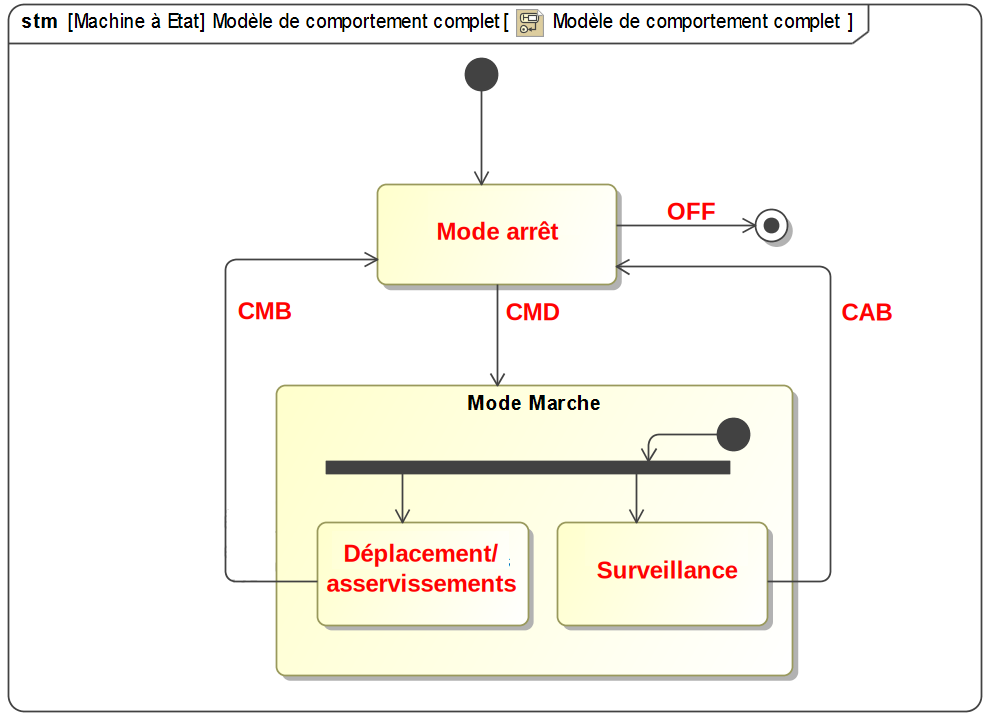
\includegraphics[width=0.8\linewidth]{img/dr02_cor}\end{center}}

\ifdef{\public}{\newpage}

\reponse{0}{\begin{center}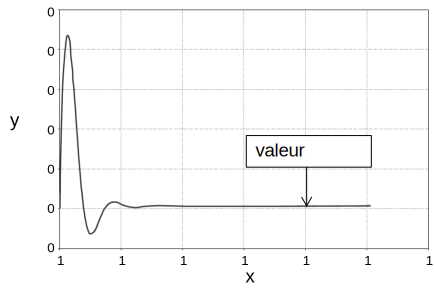
\includegraphics[width=0.5\linewidth]{img/fig11}\end{center}}{\begin{center}
  \resizebox{0.5\textwidth}{!}{\input{img/fig11_cor.pdf_tex}}
\end{center}}

\reponse{0}{\begin{center}
  \resizebox{0.6\textwidth}{!}{\input{img/dr03.pdf_tex}}
\end{center}}{\begin{center}
  \resizebox{0.6\textwidth}{!}{\input{img/dr03_cor.pdf_tex}}
\end{center}}

\reponse{0}{\begin{center}\includegraphics[width=0.5\linewidth]{img/dr04}\end{center}}{\begin{center}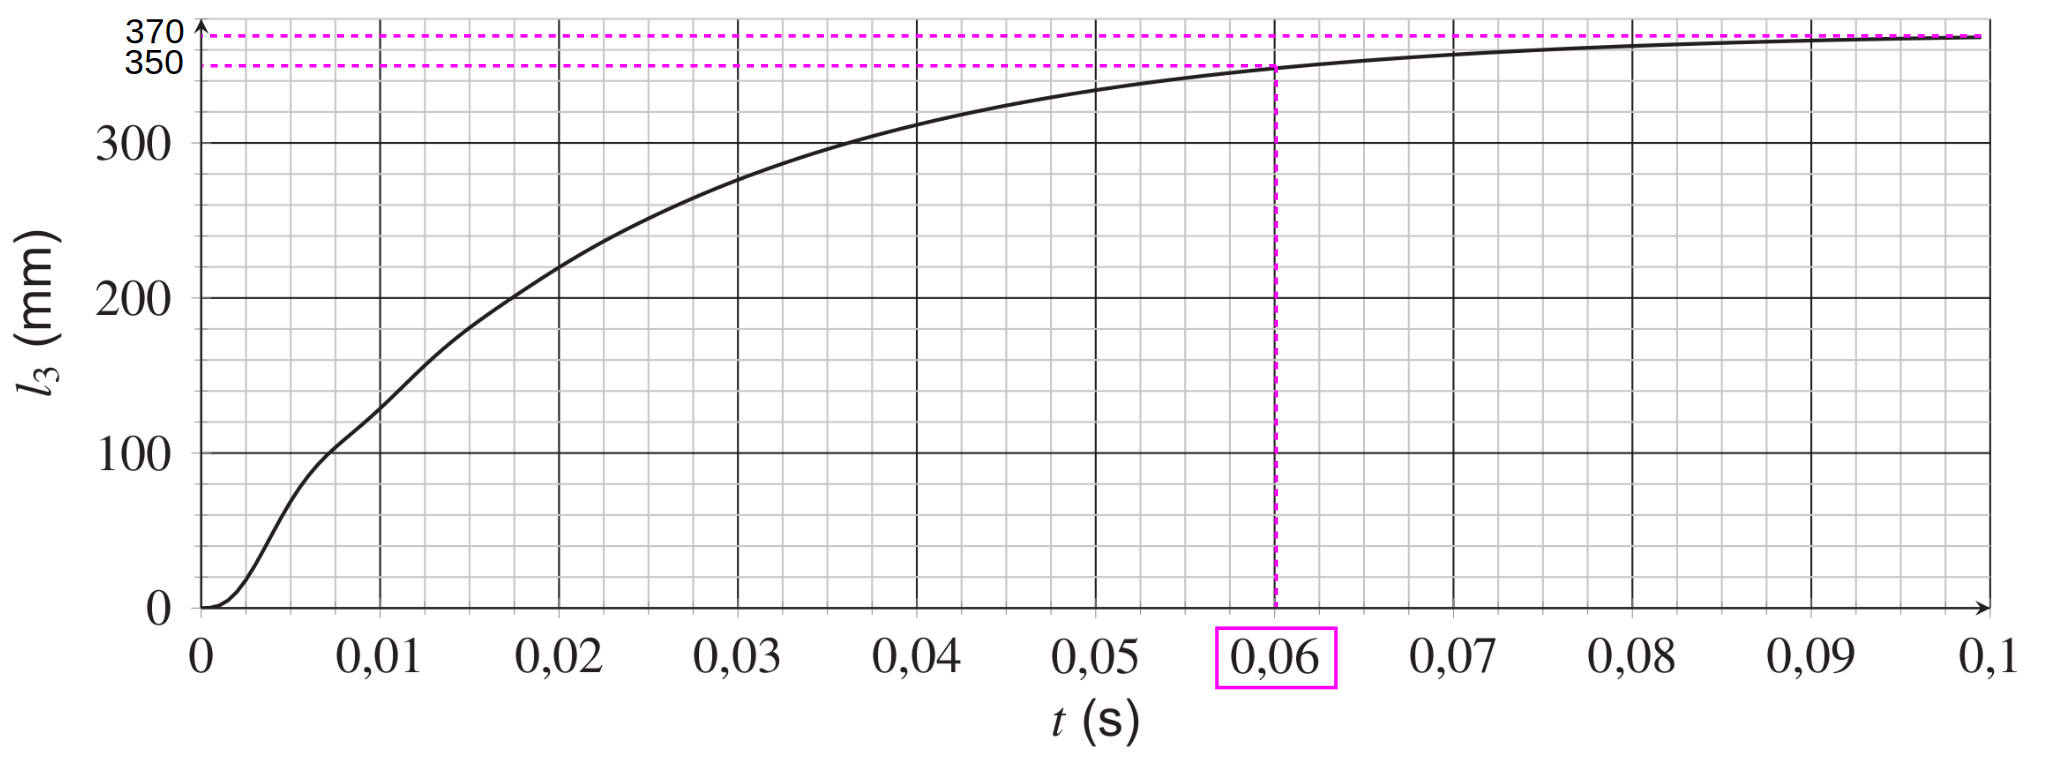
\includegraphics[width=0.5\linewidth]{img/dr04_cor}\end{center}}

\reponse{3}{}{La fréquence de coupure est 200Hz, donc $\tau=\frac{1}{2\cdot\pi\cdot f_0}=\frac{1}{2\cdot\pi 200}\approx 796\mu s$}

\reponse{1}{}{$K_a=c$}

\reponse{1}{\begin{center}\includegraphics[width=0.7\linewidth]{img/dr05}\end{center}}{$H_{bo}(j\omega)=\frac{abc}{j\omega\left(1+\tau j\omega\right)}=\frac{1777}{j\omega\left(1+\frac{j\omega}{1256}\right)}$ avec $\omega_c=1256rad\cdot s^{-1}$ et $\omega_{c,G}\approx 0$
\begin{center}
  \resizebox{0.8\textwidth}{!}{\input{img/dr05_cor.pdf_tex}}
\end{center}}

\reponse{3}{}{$\mu(p)=\theta_c(p)-\theta(p)$, donc $\mu(p)=\frac{\theta_c(p)}{1+H_{bo}(p)}$}

\reponse{5}{}{$\mu p=\lim\limits_{p\rightarrow 0}p\frac{\theta_0}{p\left(1+H_{bo}(p)\right)}=\lim\limits_{p\rightarrow 0}\frac{\theta_0}{1+\frac{abc}{p\left(1+\tau p\right)}}=0$

$\mu v=\lim\limits_{p\rightarrow 0}p\frac{\omega_0}{p^2\left(1+H_{bo}(p)\right)}=\lim\limits_{p\rightarrow 0}\frac{\omega_0}{p+p\frac{abc}{p\left(1+\tau p\right)}}=\frac{\omega_0}{abc}$

$\frac{1}{abc}=\frac{1}{0,0434\cdot 31,4\cdot 1304}\approx 0,056\%<0.1\%$}

\reponse{0}{\begin{center}\includegraphics[width=0.8\linewidth]{img/dr06}\end{center}}{\begin{center}
  \resizebox{0.8\textwidth}{!}{\input{img/dr06_cor.pdf_tex}}
\end{center}}

\reponse{5}{}{Les efforts sont situés entre les roulements donc montage en X. La bague extérieure voit la charge tournante, donc il faut serrer sur l'alésage.}

\ifdef{\public}{\newpage}

\reponse[3]{0}{\begin{center}
  \resizebox{0.5\textwidth}{!}{\input{img/dr07.pdf_tex}}
\end{center}}{\begin{center}
  \resizebox{0.5\textwidth}{!}{\input{img/dr07_cor.pdf_tex}}
\end{center}}
\end{document}
